% !TEX TS-program = xelatex
% !TEX encoding = UTF-8 Unicode
% !Mode:: "TeX:UTF-8"

\documentclass{resume}
\usepackage{tabu}
\usepackage{multirow}
\usepackage{progressbar}
\usepackage{zh_CN-Adobefonts_external} % Simplified Chinese Support using external fonts (./fonts/zh_CN-Adobe/)
% \usepackage{NotoSansSC_external}
% \usepackage{NotoSerifCJKsc_external}
% \usepackage{zh_CN-Adobefonts_internal} % Simplified Chinese Support using system fonts
\usepackage{linespacing_fix} % disable extra space before next section
\usepackage{cite}

\begin{document}
\pagenumbering{gobble} % suppress displaying page number

\Large{
  \begin{tabu}{ c l r }
    \multirow{4}{1in}{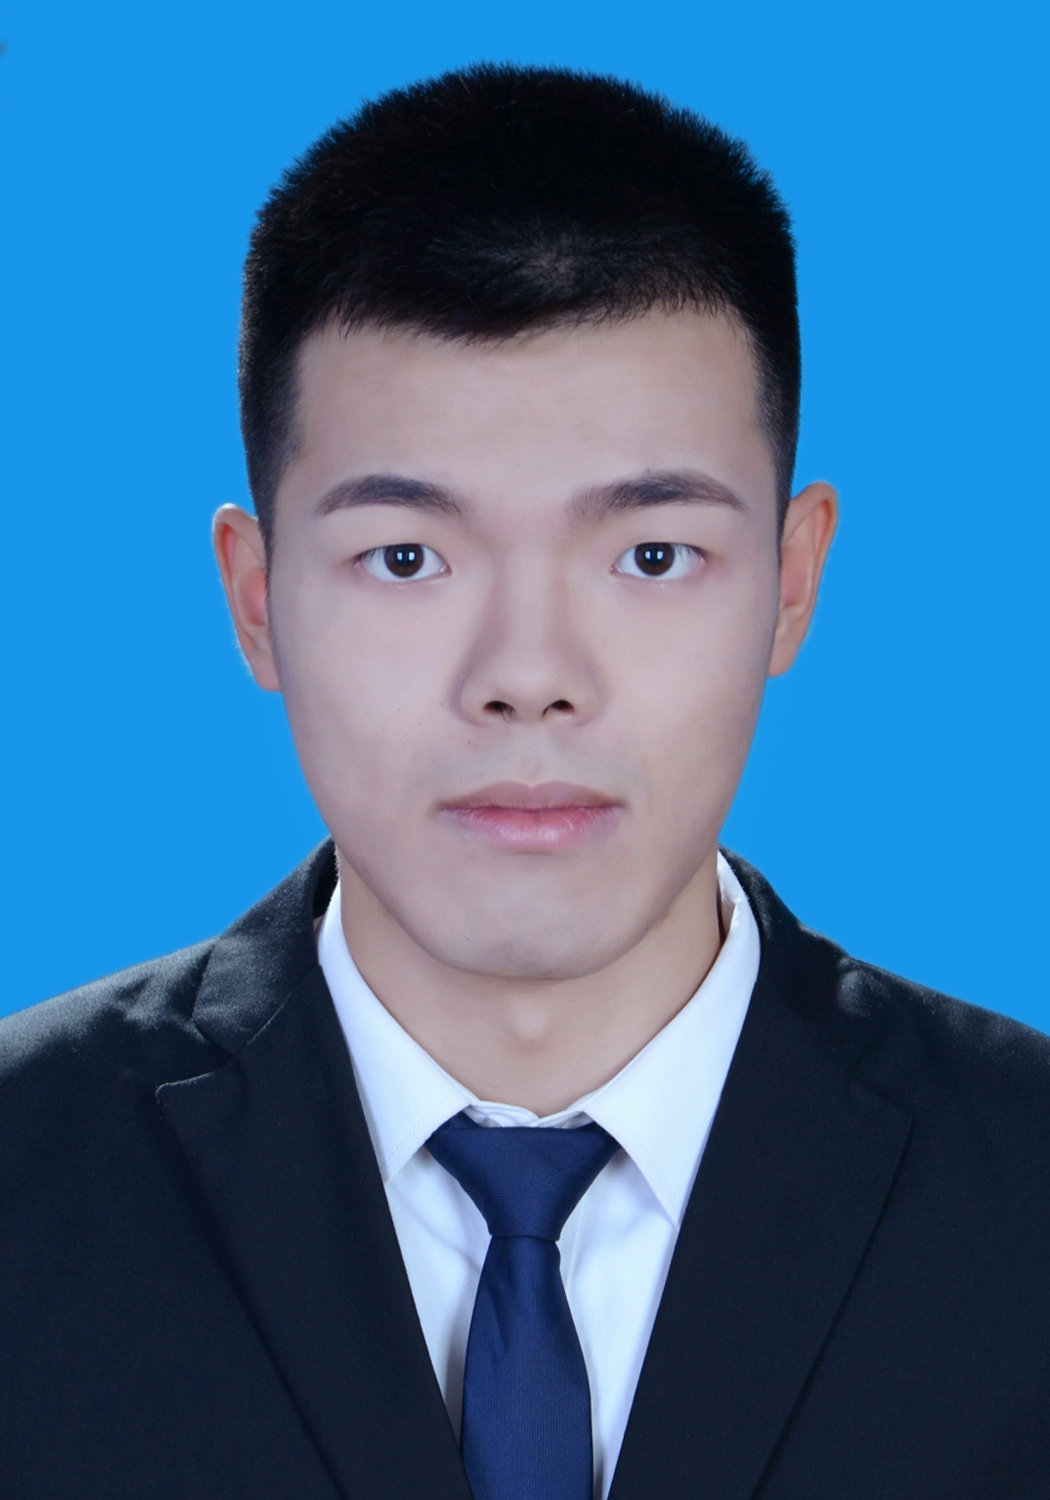
\includegraphics[width=0.8in]{photo.jpg}} & \scshape{李典源} & {C\/ C++~}\progressbar{0.75} \\
    & \phone{(+86) 156-597-72771} & {Java~}\progressbar{0.5} \\
    & \email{maybeldy@foxmail.com} & {Typescript~}\progressbar{0.75} \\
    & \github[github.com/lidotcircle]{https://github.com/lidotcircle} & {Python~}\progressbar{0.5}
  \end{tabu}
}
\vskip 1.5em
\large

%\name{李典源}
%\basicInfo{
%  \email{maybeldy@foxmail.com} \textperiodcentered\ 
%  \phone{(+86) 156-59-772771} \textperiodcentered\ 
%}
 
\section{\faGraduationCap\  教育背景}
\datedsubsection{\textbf{福州大学}, 福州}{2020 -- 至今}
\textit{在读硕士研究生}\ 电子信息(计算机技术), 预计 2023 年 6 月毕业
\datedsubsection{\textbf{福州大学},福州}{2015 -- 2019}
\textit{学士}\ 土木工程

\section{\faUsers\ 实习/项目经历}
\datedsubsection{\textbf{Socks5代理}}{2020年4月 -- 至今}
\role{C/C++, Vue}{个人项目}
\begin{onehalfspacing}
前端、后端开发, https://github.com/lidotcircle/hula
\begin{itemize}
  \item Socks5代理
  \item 客户端和服务端之间通信使用TLS加密
  \item 复用TLS链接, 减少TLS握手的开销
\end{itemize}
\end{onehalfspacing}

\datedsubsection{\textbf{简易网盘}}{2020年3月 -- 至今}
\role{Typescript, Angular, Docker}{个人项目}
\begin{onehalfspacing}
前端、后端开发, https://github.com/lidotcircle/webdisk
\begin{itemize}
  \item 基于Web的网盘管理页面
  \item 多用户的文件访问控制
  \item 支持多种后端的储存方式(硬盘、OSS)
  \item HTTP协议链接的离线下载
\end{itemize}
\end{onehalfspacing}

% Reference Test
%\datedsubsection{\textbf{Paper Title\cite{zaharia2012resilient}}}{May. 2015}
%An xxx optimized for xxx\cite{verma2015large}
%\begin{itemize}
%  \item main contribution
%\end{itemize}

\section{\faCogs\ IT 技能}
% increase linespacing [parsep=0.5ex]
\begin{itemize}[parsep=0.5ex]
  \item 编程语言: C/C++ == Typescript > Java == Rust == Python
  \item 前端框架: Angular
  \item 后端开发: Spring Boot
  \item 区块链: Hyperledger Fabric
  \item 平台: Linux
  \item 开发工具: Git, Docker
\end{itemize}

\section{\faArrowCircleRight\ 自我评价}
做事耐心, 喜欢学习新技术和新知识, 热爱编程.

\section{\faInfo\ 其他}
% increase linespacing [parsep=0.5ex]
\begin{itemize}[parsep=0.5ex]
  \item 技术博客: http://lidotcircle.ltd
%  \item GitHub: https://github.com/lidotcircle
  \item 语言: 英语 (CET-6)
\end{itemize}

%% Reference
%\newpage
%\bibliographystyle{IEEETran}
%\bibliography{mycite}
\end{document}
